% Default compiler: lualatex
% Default bibliography tool: biber
% Bibliography->Type= BibTex

\documentclass[a4paper,11pt,oneside]{memoir}
%!TEX root = main.tex
% Encoding
%\usepackage[utf8]{inputenc} % pdfLatex
\usepackage[T1]{fontenc}
\usepackage[danish]{babel}
\renewcommand{\danishhyphenmins}{22}
\usepackage[utf8]{inputenc} % æ ø å

% Date
\usepackage[ddmmyyyy]{datetime}
\renewcommand{\dateseparator}{.}

% Fonts
\usepackage{fourier}
\usepackage[scaled=0.8]{beramono}

% Math
\usepackage{amsmath,amssymb}
\usepackage{bm}
\usepackage{amsthm}
\usepackage{mathtools}

% Graphics
\usepackage[usenames,dvipsnames,table]{xcolor}
\usepackage{graphicx}
\usepackage{float}
%\usepackage[section]{placeins}
\usepackage{tikz}
\usepackage[pages=some]{background}
\usepackage{wrapfig}

% Listings & Tables
\usepackage{listings}
%\usepackage{pythontex}
\usepackage{enumitem}
\usepackage{tabu}
\usepackage{longtable}
\usepackage{multirow}
\usepackage{makecell}
\usepackage{booktabs}
\setlength{\tabcolsep}{10pt}
\renewcommand{\arraystretch}{1.2}


% References & Quotes
\usepackage[danish]{varioref}				% Muliggoer bl.a. krydshenvisninger med sidetal (\vref)
%\usepackage{nat}							% Udvidelse med naturvidenskabelige citationsmodeller
\usepackage[perpage]{footmisc}	% resets footnote counter on new page
\usepackage[danish=guillemets]{csquotes}
\usepackage[hidelinks]{hyperref}
\hypersetup{
    pdfstartview={FitH},
    pdftitle={Smart Pool 2.0},
    pdfsubject={Projektrapport},
    pdfauthor={I4PRJ4GRP3}
}
\usepackage[all]{hypcap}

% Etc
\usepackage{todonotes} % "to-do"-liste vha. \todo{opgave}
\usepackage[
	backend=biber,
	%backend=bibtex,
	style=ieee,
	natbib=true,
	backref=false,
	backrefstyle=all+,
	hyperref=true
]{biblatex}
\usepackage{pdflscape}
\usepackage[nomain,toc,xindy,acronym,nonumberlist,noredefwarn]{glossaries}
\usepackage[xindy]{imakeidx}
\usepackage{float}
\makeindex

%=== Indstillinger til kodestykker ==========================%
%\usepackage{listings} % kode
%\lstset{
%	language = C++, 
%	backgroundcolor=\color{black!5},
%	basicstyle=\footnotesize,
%	commentstyle=\color{mygreen},
%	frame=single, 						% laver en ramme om koden
%	keepspaces=true, 					% beholde indrykning
%	keywordstyle=\color{blue},
%	numbers=left, 
%	numbersep=2pt, 						% afstand fra nummer til kode
%	numberstyle=\color{mygray}, 		% linjenummer farve
%	stringstyle=\color{green!70!black}, 		% string farve
%	tabsize=5,
%	captionpos=b, % sets the caption-position to bottom
%	otherkeywords={null}, 	% til keywords 
%	showstringspaces=false
%}
\renewcommand\lstlistingname{Code listing}

\definecolor{bluekeywords}{rgb}{0,0,1}
\definecolor{greencomments}{rgb}{0,0.5,0}
\definecolor{redstrings}{rgb}{0.64,0.08,0.08}
\definecolor{xmlcomments}{rgb}{0.5,0.5,0.5}
\definecolor{types}{rgb}{0.17,0.57,0.68}

\usepackage{listings}
\lstset{language=[Sharp]C,
	captionpos=b,
	numbers=left, %Nummerierung
	numberstyle=\tiny, % kleine Zeilennummern
	frame=lines, % Oberhalb und unterhalb des Listings ist eine Linie
	showspaces=false,
	showtabs=false,
	breaklines=true,
	showstringspaces=false,
	breakatwhitespace=true,
	escapeinside={(*@}{@*)},
	commentstyle=\color{greencomments},
	morekeywords={partial, var, value, get, set},
	keywordstyle=\color{bluekeywords},
	stringstyle=\color{redstrings},
	%basicstyle=\ttfamily\small,
}

% Dummy
\usepackage{lipsum}
%!TEX root = main.tex
% Page setup
\setulmarginsandblock{35mm}{25mm}{*}
\setlrmarginsandblock{20mm}{20mm}{*}
\setheadfoot{4\onelineskip}{2\onelineskip}
\setheaderspaces{*}{5mm}{*}
\checkandfixthelayout

% Pagestyle
\makepagestyle{asereport}
	\makeevenhead{asereport}{}{}{}
	\makeoddhead{asereport}{
\includegraphics{figs/frontpage/aseaulogo.pdf}}{}{\small\rightmark{} | \textbf{\thepage{}\vspace{7pt}}}
	\makeevenfoot{asereport}{}{}{}
	\makeoddfoot{asereport}{}{}{}

\makepsmarks{asereport}{
	\createmark{chapter}{both}{shownumber}{}{. \ }
	\createmark{section}{both}{shownumber}{}{. \ }
	\createmark{subsection}{both}{shownumber}{}{. \ }
	\createplainmark{toc}{both}{\contentsname}
	\createplainmark{lof}{both}{\listfigurename}
	\createplainmark{lot}{both}{\listtablename}
	\createplainmark{bib}{both}{\bibname}
	\createplainmark{index}{both}{\indexname}
	\createplainmark{glossary}{both}{\glossaryname}
}

\aliaspagestyle{part}{asereport}
\aliaspagestyle{chapter}{asereport}
\chapterstyle{tandh}

% Modification to certain spacing
\setlength{\parskip}{8pt}
\setlength{\parindent}{0pt}
\setlength{\abovecaptionskip}{7pt}
\setlength{\belowcaptionskip}{-10pt}
\OnehalfSpacing

% Tabu
%\taburowcolors[1]2{white .. light-gray}
\tabulinesep=4pt

% Itemize/enumerate
\setlist{
    before=\vspace{-3pt}, 
    after=\vspace{-3pt},
    itemsep=0pt,
    leftmargin=25pt,
    labelsep=10pt,
    topsep=0pt,
}

% Kommandoer til UC - fixer spacing
% Aktører
\newcommand{\fua}[1]{
	\begin{minipage}[t]{\linewidth}
		\setlist{
		    leftmargin=22pt,
		    itemsep=0pt,
		    topsep=0pt,
		    parsep=3pt
		}
	\begin{itemize}[before={\vspace{-6pt}}, after={\vspace{6pt}}]
	#1
	\end{itemize}
	\end{minipage}
}

% Hovedforløb
\newcommand{\fu}[1]{
\begin{minipage}[t]{\linewidth}
\setlist{
    leftmargin=22pt,
    itemsep=0pt,
    topsep=0pt,
    parsep=3pt
}
\raggedright
\begin{enumerate}[before={\vspace{-5pt}},after={\vspace{6pt}}]
#1
\end{enumerate}
\end{minipage}}

% Extensions
\newcommand{\fuex}[2]{
\begin{minipage}[t]{\linewidth}
\vspace{-6pt}
\raggedright
\textit{#1}
\begin{enumerate}[leftmargin=22pt,itemsep=0pt,parsep=3pt,before={\vspace{-8pt}}, after={\vspace{20pt}},topsep=8pt]
#2
\end{enumerate}
\end{minipage}
}

% Extensions - Sidste entry
\newcommand{\fuexl}[2]{
\begin{minipage}[t]{\linewidth}
\vspace{-6pt}
\raggedright
\textit{#1}
\begin{enumerate}[leftmargin=22pt,itemsep=0pt,parsep=3pt,before={\vspace{-8pt}}, after={\vspace{3pt}},topsep=8pt]
#2
\end{enumerate}
\end{minipage}}

% Versionshistorik
\newcommand{\verhistitem}[2]{
\begin{minipage}[t]{\linewidth}
\vspace{-6pt}
\raggedright
#1
\begin{itemize}[leftmargin=22pt,itemsep=0pt,parsep=0pt,before={\vspace{-10pt}},after={\vspace{3pt}},topsep=8pt]
#2
\end{itemize}
\end{minipage}}

\newcommand{\tverb}[1]{{\texttt{#1}}}

\newcommand{\cond}[1]{
\begin{itemize}[label=,noitemsep,topsep=0pt,after={\vspace*{-\baselineskip}}]
#1
\end{itemize}}

% Etc
\definecolor{light-gray}{gray}{0.8}
\definecolor{pantone}{RGB}{0,61,133}

\setfloatlocations{figure}{H}
\setfloatlocations{table}{H}

\numberwithin{equation}{chapter}
\numberwithin{figure}{chapter}
\setcounter{secnumdepth}{2}
\setcounter{tocdepth}{2}
\maxsecnumdepth{subsection}

\renewcommand*{\cftdotsep}{1}
\setpnumwidth{2em}
\setrmarg{2em}

\setverbatimfont{\ttfamily}

%\renewcommand\cftchaptername {\chaptername~}
%\renewcommand\cftappendixname {\appendixname~}
\addto\captionsdanish{
    \renewcommand\contentsname{Indholdsfortegnelse}
    \renewcommand\appendixname{Appendiks}
}
\renewcommand\appendixpagename{Appendiks}
\renewcommand\appendixtocname{Appendiks}
\newsubfloat{figure}

% Abstract
\newenvironment{abstracten}
{\renewcommand{\abstractname}{Abstract}\abstract}
{\endabstract}
\renewcommand{\abstractnamefont}{\normalfont\Large\bfseries}
%!TEX root = main.tex
% Listings
\AtBeginDocument{%
  \counterwithin*{lstlisting}{section}
  \counterwithin*{lstlisting}{subsection}
  \counterwithin*{lstlisting}{subsubsection}
  \renewcommand{\thelstlisting}{%
    \ifnum\value{subsection}=0
      \thesection.\arabic{lstlisting}%
    \else
      \ifnum\value{subsubsection}=0
        \thesubsection.\arabic{lstlisting}%
      \else
        \thesubsubsection.\arabic{lstlisting}%
      \fi
    \fi
  }
}

% Loading languages
\lstloadlanguages{C, C++}

% Listing setup
\lstdefinestyle{all}{
    basicstyle    = \ttfamily\SingleSpacing\scriptsize,
    numbers       = left, 
    numberstyle   = \ttfamily\tiny,
    breaklines    = true,
    commentstyle=\color{green},
    %backgroundcolor = \color{red},
    numbersep     = 20pt,
    xleftmargin   = \parindent,
    captionpos    = b,
    keywordstyle  = [1]\color{Blue}\bfseries,
    commentstyle  = \itshape\color{Green},
    tabsize       = 3
}

\lstset{
    style = all
} 
%!TEX root = main.tex
\makenoidxglossaries

\newglossaryentry{smartpool}{
	name={Smartpool}, 
	description={Navnet på projektet og systemet.}
}

\newglossaryentry{dotcover}{
	name={DotCover}, 
	description={Lavet af JetBrains. dotCover er et .NET test-runner og code coverage værktøj - \url{https://www.jetbrains.com/dotcover/}}
}

\newglossaryentry{UIKit}{
	name={UIKit},
	description={GUI framework til iOS udvikling. Indeholder klasser som UITableViewControl}
}

\newglossaryentry{ef}{
	name={Entity Framework}, 
	description={Framework til object orienteret adgang til en database.}
}

\newglossaryentry{windserver}{
	name={Connection Server}, 
	description={Del af systemet som modtager requests fra brugeren.}
}

\newglossaryentry{gui}{
    name={GUI}, 
    description={Graphical User Interface er en brugergrænseflade. Brugerens måde at tilgå systemet på}
}

\newglossaryentry{us}{
	name={User stories}, 
	description={User stories er en metode til at specificere de funktionelle krav til et system.}
}

\newglossaryentry{iosapp}{
	name={iOS-applikation}, 
	description={Et program der med et GUI tillader brugeren at bruge systemet fra en iPhone.}
}

\newglossaryentry{webapp}{
	name={Web-applikation}, 
	description={Et program der med et GUI tillader brugeren at bruge systemet fra en internet browser på alle platforme.}
}

\newglossaryentry{pcapp}{
	name={PC-applikation}, 
	description={Et program der med et GUI tillader brugeren at bruge systemet fra en Windows PC.}
}

\newglossaryentry{moscow}{
    name={MoSCoW}, 
    description={MoSCoW er en metode til at prioritere krav til ens system}
}

% muligvis ikke nødvendig
\newglossaryentry{user}{
		name={User},
		description={Bruger eller kunde. Brugeren der er oprettet i systemet eller brugeren, der har en pool.}
}
	
\newglossaryentry{admin}{
	name={Administrator},
	description={En ansat der kan tilgå databasen og direkte ændre på den i tilfælde af fejl.}
}

\newglossaryentry{tv}{
	name={Target-værdier},
	description={De ønskede værdier for de forskellige mål i poolen, som f.eks. temperatur.}
}

\newglossaryentry{mu}{
	name={MonitorUnit},
	description={Fysisk enhed med sensorer der installeres i poolen. Kan også referere til entitet på databasen, som indeholder målingerne fra den fysiske MoniterUnit}
}

\newglossaryentry{specinvite}{
	name={Spectate invitation},
	description={En måde hvorpå en bruger tillader en anden bruger at blive spectator af én af sine pools.}
}

\newglossaryentry{spectator}{
	name={Spectator},
	description={En bruger i systemet, som kan se en pool, men ikke ændre på den, da den tilhører en anden bruger.}
}

\newglossaryentry{nunit}{
	name={NUnit},
	description={Unittest framework til .NET - \url{http://www.nunit.org/}}
}

\newglossaryentry{nsub}{
	name={NSubstitute},
	description={Mocking framework til .NET - \url{http://nsubstitute.github.io/}}
}

\newglossaryentry{db}{
	name={Database},
	description={Relational database. En server der indeholder alt data i systemet.}
}

\newglossaryentry{pool}{
	name={Pool},
	description={Swimming pool hvor i produktet kan installeres.}
}

\newglossaryentry{Microsoft .NET}{
	name={Microsoft .NET},
	description={Microsoft's .NET-framework er blevet brugt i udviklingen af de meste af sourcekoden i projektet.}
}

\newglossaryentry{NUnit}{
	name={NUnit},
	description={Er et test framework som er anvendt til at skrive automatiske tests}
}

\newglossaryentry{NSubstitute}{
	name={NSubstitute},
	description={Er et mocking bibliotek der anvendes til at generere fakes til tests i NUnit}
}

\newglossaryentry{WPF}{
	name={WPF},
	description={WPF-framework'et er blevet brugt til udviklingen af systemets Windows brugergrænseflade.}
}

\newglossaryentry{ASP.NET MVC}{
	name={ASP.NET MVC},
	description={ASP.NET MVC er et framework, der er blevet brugt, til udviklingen af Web-applikationen.}
}

\newglossaryentry{NUnit Testframework}{
	name={NUnit Testframework},
	description={Et oplagt værktøj til softwaretest har været Nunit idet det bruges i vid udstrækning i forbindelse med kurset Software Test.}
}

\newglossaryentry{ADO.NET Entity}{
	name={ADO.NET Entity},
	description={ADO.NET Entity-framework'et er brugt til implementeringen af data-access laget. Framework'et er brugt for at muliggøre objektorienteret interaktion med systemets database.}
}





%% Forside variabler
\newcommand{\Kursus}{I4PRJ4 F16}
\newcommand{\Projektnavn}{SmartPool 2.0}
\newcommand{\Gruppe}{Gruppe 3}
\newcommand{\Projektdokument}{Projektrapport}

\bibliography{../utils/litteratur.bib} %% Litteratur

\begin{document}		
	\frontmatter
	\pagestyle{asereport}
	%!TEX root = main.tex
\pagestyle{titlingpage}
\backgroundsetup{
	scale=1,
	angle=0,
	opacity=1,
	contents={
		\begin{tikzpicture}[remember picture,overlay]
		\path [fill=pantone] (-0.5\paperwidth,0.36\paperheight) rectangle (0.5\paperwidth,0.47\paperheight);  
		\path [fill=pantone] (-0.5\paperwidth,-0.47\paperheight) rectangle (0.5\paperwidth,-0.43\paperheight);  
		\end{tikzpicture}}}
\BgThispage
\vspace*{-25mm}
\begin{minipage}[l]{\textwidth}
	
\includegraphics[width=0.75\textwidth]{figs/frontpage/aseaulogohvid.pdf}
\end{minipage}

\vspace{35pt}
\begin{minipage}[l]{\textwidth}
\tabulinesep=10pt
\begin{tabu} to \textwidth{X[l]}
	{\small\MakeUppercase\Kursus}\\
	{\HUGE\bfseries\MakeUppercase\Projektnavn}\\
	{\Large\Gruppe}\\
	{\itshape\Projektdokument}
\end{tabu}
\end{minipage}

\vspace{5pt}
\begin{minipage}[l]{\textwidth}
    \centering
	\vspace*{0cm}\hspace*{8cm}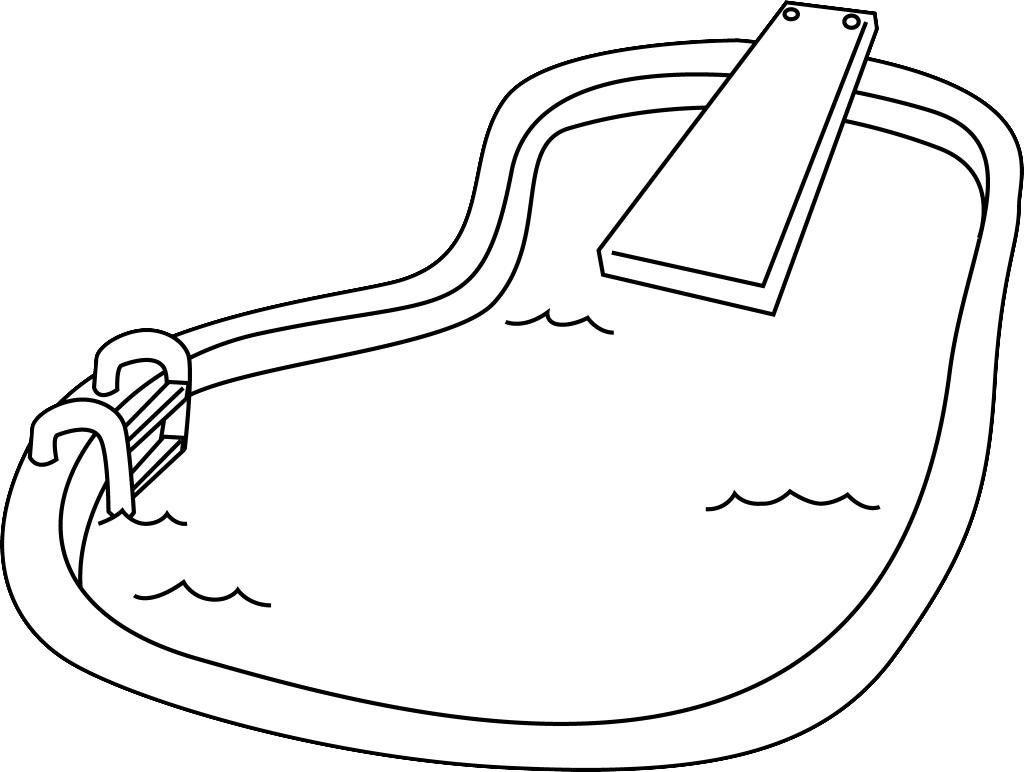
\includegraphics[width=0.4\textwidth]{figs/frontpage/smartpool.png}
\end{minipage}

\vspace{\fill}
\begin{minipage}[l]{\textwidth}
\begin{tabu} to \textwidth{lX[l]}
\textbf{Dato}           &\today\\
\textbf{Vejleder}		&Vejleder navn\\
\end{tabu}
\end{minipage}

\vspace{10pt}
\begin{minipage}[l]{\textwidth}
\tabulinesep=25pt
\begin{tabu} to \textwidth{X[l]X[l]X[l]}
 \makebox[\linewidth]{\hrulefill}\newline Joachim Dam Andersen     \newline 201370248/IKT  
&\makebox[\linewidth]{\hrulefill}\newline Lasse Priebe             \newline 201370248/IKT 
&\makebox[\linewidth]{\hrulefill}\newline Emil Nyborg              \newline 201370248/IKT\\
 \makebox[\linewidth]{\hrulefill}\newline Bjørn Nørgaard Sørensen  \newline 201370248/IKT  
&\makebox[\linewidth]{\hrulefill}\newline Alex Justesen Karlsen    \newline 201370248/IKT 
&\makebox[\linewidth]{\hrulefill}\newline Joachim Händel Noer Wind \newline 201370248/IKT
\end{tabu}
\end{minipage}					\clearpage %% Forside
	% Initial setup
\markboth{RESUMÉ/ABSTRACT}{RESUMÉ/ABSTRACT}
\abstractintoc
\abstractcol
\setlength{\abstitleskip}{-18pt}

% Abstract
\begin{abstract}
\lipsum[3-4] %% danske abstrakt skrives her
\end{abstract}

\begin{abstracten}
\lipsum[3-4] %% english abstract goes here
\end{abstracten}		\clearpage %% Abstract
	\chapter{Forord}

% Forordet benyttes til at informere kort om visse ydre omstændigheder for projektet, såsom projekttype og hvor projektet er gennemført, historisk baggrund (andre arbejder, som har givet anledning til det aktuelle projekt) og hvor inspirationen og ideen er kommet fra, m.v.

Dette dokument er sammensat for at dokumentere arbejdet på 4. semesterprojektet for retningen IKT på ingeniørhøjskolen Århus.

Der vil i denne rapport være referencer til bilag og dokumentation, som det ikke ville være hensigtsmæssigt at medtage. Samtlige bilag m.m. vil være at finde på den vedlagt CD-rom. 

Source kode til projektet kan findes på CD'en. Link til vores github repo følger her: \newline \url{https://github.com/joachimda/I4PRJ}

\vspace{5mm}

\large{\textit{En stor tak til}}

\begin{displayquote}
    Lars Mortensen for god og brugbar vejledning.
\end{displayquote}

\begin{displayquote}
   Underviserne på ASE, for hjælp og vejledning.
\end{displayquote}

			\clearpage %% Forord
	\tableofcontents						\clearpage %% ToC
	
	\mainmatter
	%\listoftodos[Liste over gøremål]%% Todo oversigt - SKAL UDKOMMENTERES FØR AFLEVERING
	\chapter{Indledning}

%% indledning goes here.

Dokumentet er projektdokumentation af projekt gruppe 9 i kurset I4PRJ4 på Ingeniør Højskolen, Århus 
Universitet. Dokumentationen beskriver projektudviklingen for Smartpool systemet. 
Smartpool er et system, som ved hjælp af sensorer kan måle forhold for en swimmingpool. Målingerne kan 
præsenteres for en bruger vha. softwareapplikationer. Systemet kan ikke måle eller præsenterer reel data, da det i projektafgrænsningen er fravalgt. 
Dokumentationen bringer en detaljeret beskrivelse af krav til systemet, softwarearkitektur, og design af software. 
Designet implementeres og testes. Systemet integreres modul for modul. Slutteligt udføres en på forhånd defineret accepttest. 
Projektoplæg, -afgrænsning og -beskrivelse forefindes i projektrapporten. 		\clearpage %% Indledning
	\chapter{Fremtidigt arbejde}
	\clearpage %% Projektformulering
	\chapter{Fremtidigt arbejde}
		\clearpage %% Kravspecifikation
	\chapter{Fremtidigt arbejde}
	\clearpage %% Processbeskrivelse
	\chapter{Fremtidigt arbejde}
			    \clearpage %% Metodeafsnit
	\chapter{Fremtidigt arbejde}
			\clearpage %% Specifikation og analyse
	\chapter{Fremtidigt arbejde}
		\clearpage %% Arkitektur
	
	\chapter{Design og implementering}\label{cha:design}
%% indledning til kapitel skal være her...
I dette afsnit beskrives designet og implementering af software til \gls{smartpool} systemet. De forskellige ansvarsområder som applikation, forbindelse og data beskrives med indledende overvejelser. 
Designet og efterfølgende implementeringen beskrives med de to samme krav: 

\begin{itemize}
	\item Som bruger vil jeg kunne oprette mig i systemet, for at få adgang til systemet.
	\item Som bruger vil jeg kunne se de seneste sensor værdier for at kunne få et overblik over 
	poolens tilstand.
\end{itemize}

\section{Applikation}
Applikationerne i systemet er jævnfør arkitekturen lavet med MVP, og de respektive dele bliver beskrevet i rækkefølgen Model, Presenter og View. Lagets model- og præsentationslag er designet til at være portabelt, så forskellige platforme kunne dele denne kodebase. View-laget designes derimod seperat for hver platform. 

Det overordnede design i applikationslaget illustreres ved sekvensdiagrammet i figur~\ref{fig:application_sd}. Her fremgår kommunikationsmønsteret mellem model-, view- og presenter-klasserne i applikationslagets design.

\begin{figure}
	\centering
	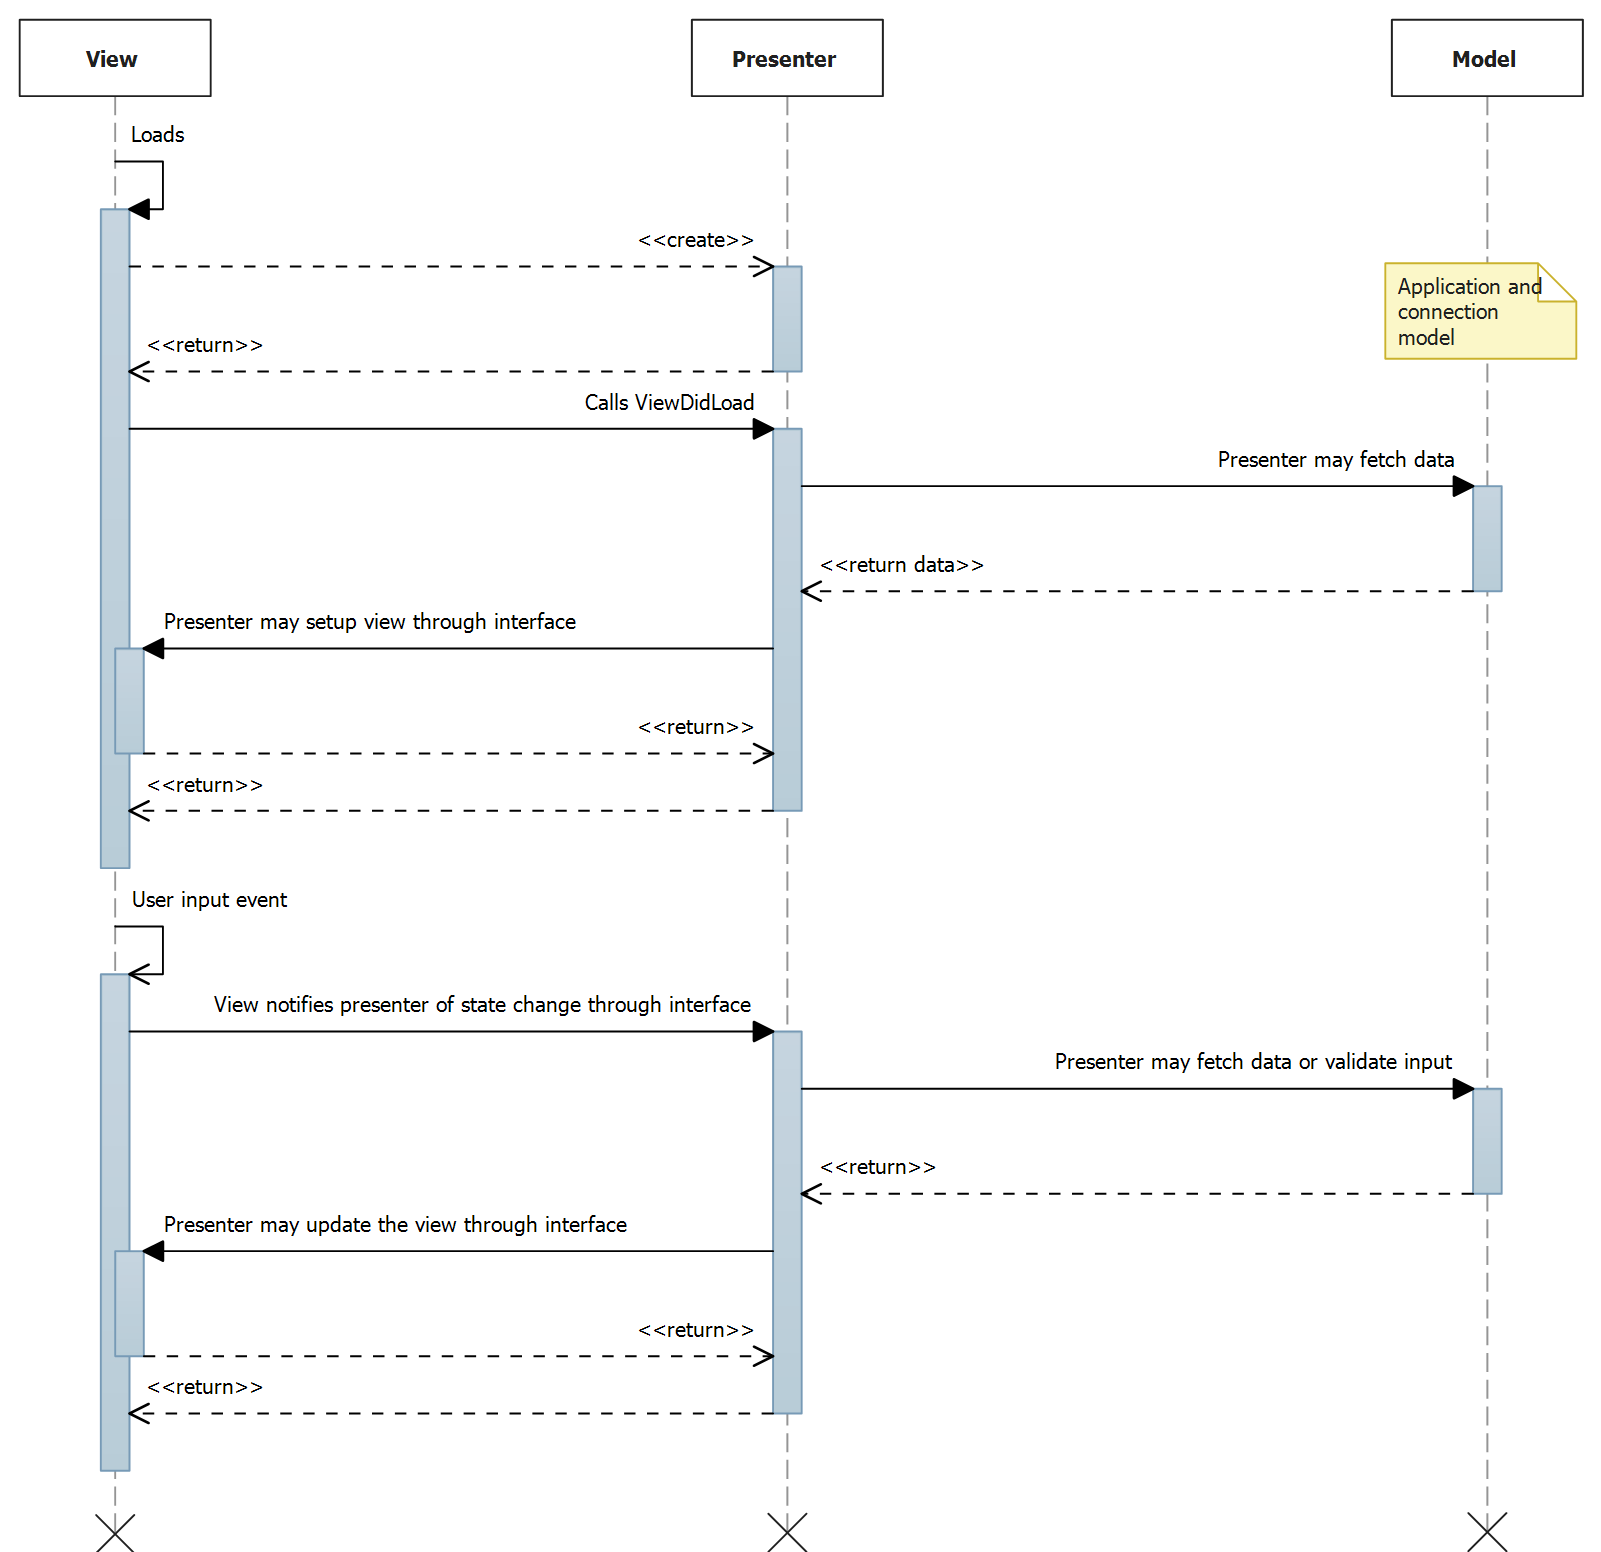
\includegraphics[width=1.0\linewidth]{figs/design/application_sd}
	\caption{Kommunikation i applikationslaget}
	\label{fig:application_sd}
\end{figure}

Som følge systemets multi-lag arkitektur kunne applikationslaget samt de platform-specifikke view-implementeringer
designes, uafhængigt af hinanden, så længe protokolbestemmende interfaces blev specificeret undervejs i processen. Interfaces for både presenters og views, er defineret ud fra de user stories, der har krævet deres design.

\chapter{Fremtidigt arbejde}

% !TEX root = ../../I4PRJ, Grp3 - Dokumentation.tex
\section{Application}\label{sec:testapplikation}
% introduktion
Applikationslaget består af et model-, view- og præsentationslag. Test-projektet: Smartpool.Application.Test indeholder en automatiseret test-suite, der tester de konkrete klasser i model- og præsentationslaget. View-implementeringen i GUI-applikationerne, er ikke mulige at teste på samme måde, og testes derfor kvalitativt.

Test-suite projektet, der tester model- og præsentationslaget, er udført med brug NUnit og NSubstitute.

\subsection{Testdetaljer}
% beskrivelse af coverage procent og antallet af test, samt begrundelse for begge.
På figur~\ref{fig:apptest} ses resultatet af de unit-tests der bliver kørt, i test-projektet: Smartpool.Application.Test. I test-suiten testes modelklasserne PoolLoader, PoolValidator, UserValidator og Session, samt en række presenter-klasser.

% BILLEDE AF KØRTE UNITTEST
\begin{figure}
\centering
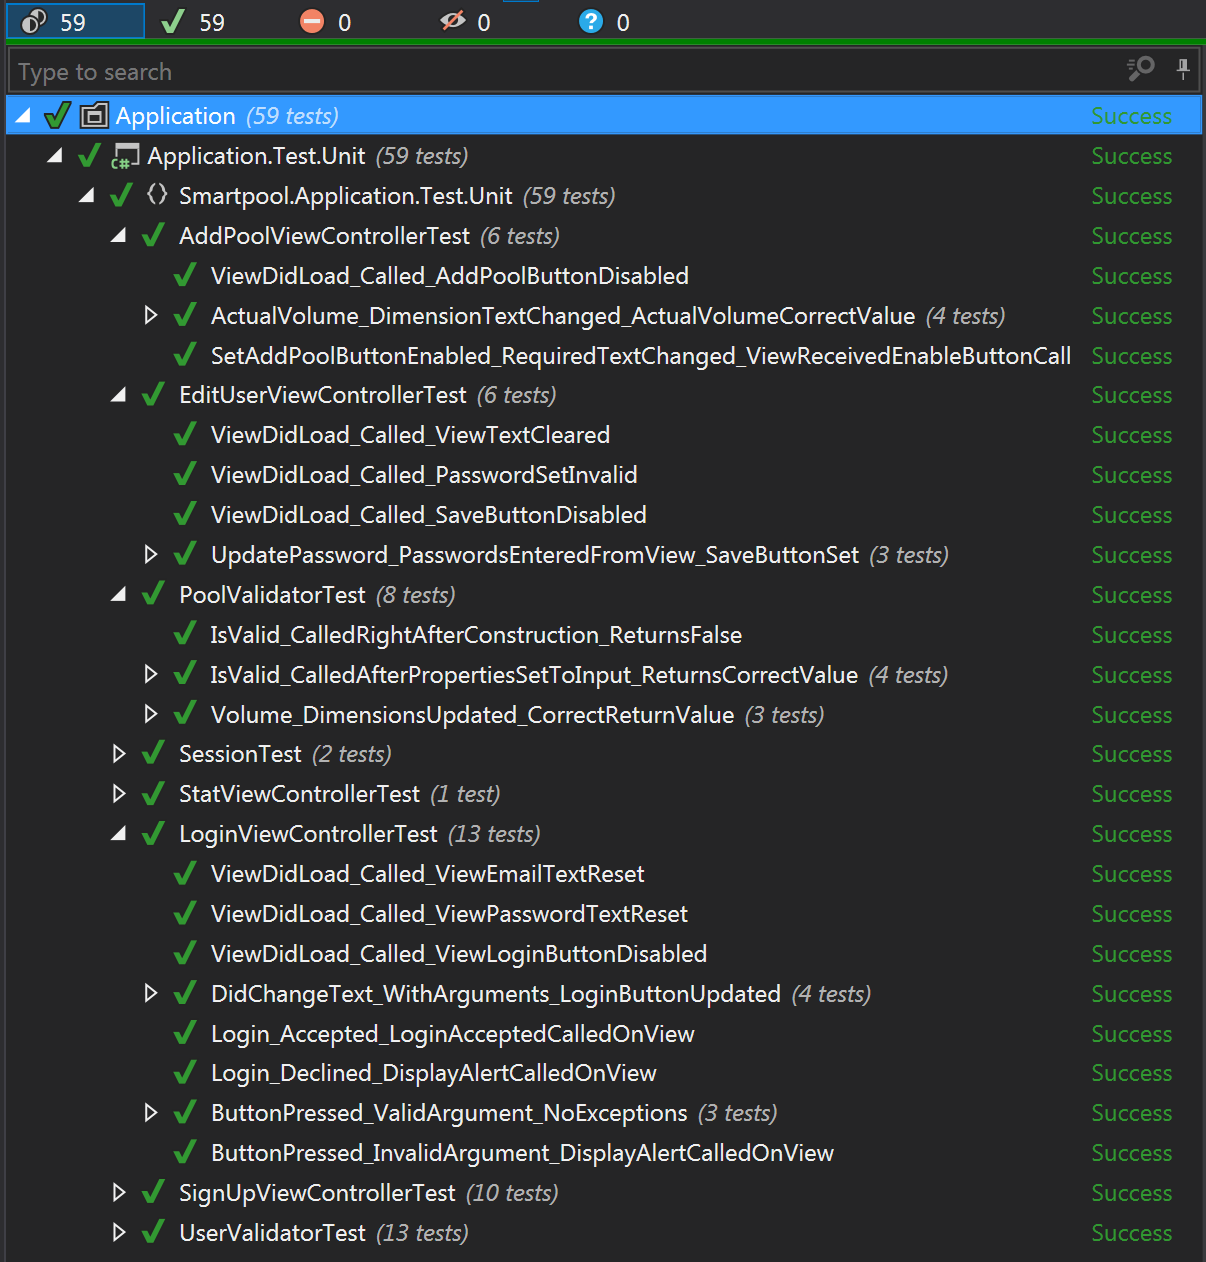
\includegraphics[width=0.9\linewidth]{figs/test/apptest}
\caption{Test af applikationslaget.}
\label{fig:apptest}
\end{figure}

I forbindelse med unit-test kører vi code coverage målinger, for at få en idé om, hvilke dele af klasserne der er testet. På figur~\ref{fig:appcoverage} ses code coverage resultatet for test-suiten. Som det fremgår af code-coverage analysen, er GUI applikationen Win (og de andre GUI applikationer), ikke testet med NUnit, og har derfor ingen code coverage.

% BILLEDE AF COVERAGE KØRT
\begin{figure}
\centering
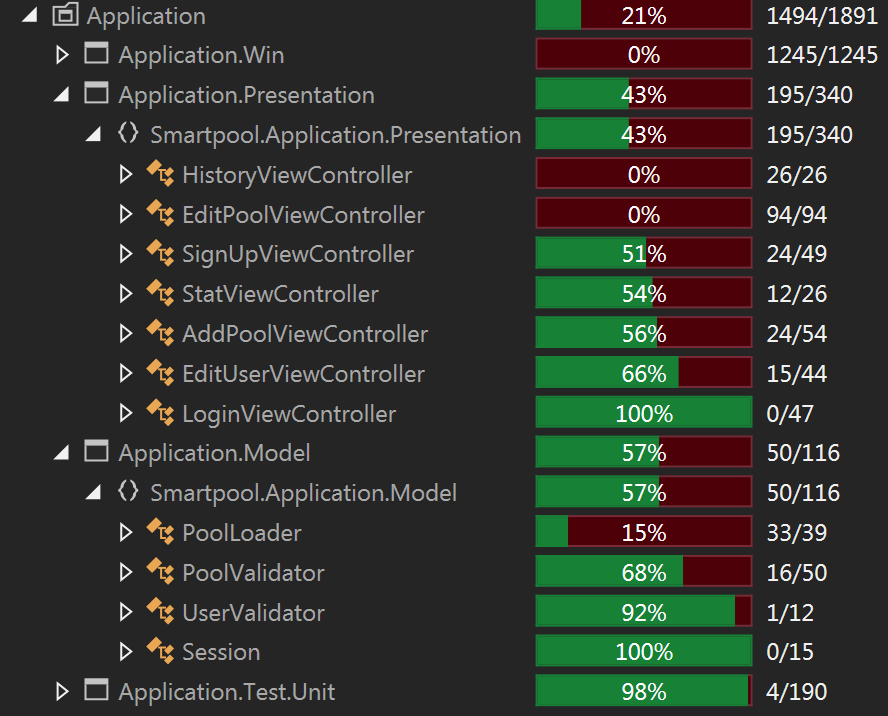
\includegraphics[width=0.9\linewidth]{figs/test/appcoverage}
\caption{Code coverage for applikationslaget.}
\label{fig:appcoverage}
\end{figure}

\subsection{Testbeskrivelse}
% hvordan div. test er valgt og hvad I specielt var opmærksom på under udviklign af test. 
% hvad var let/svært at teste etc.
Modelklasserne i applikationslaget har få afhængigheder, og kan derfor testes uden brug af fakes. Modelklasserne testes individuelt, og den ene klasse (PoolLoader) der benytter sig af en IClientMessenger, opsættes med en fake IClientMessenger. Presenter-klasserne testes også individuelt, og deres dependency til et IView og en IClientMessenger fakes med NSubstitute. I Presenter-klasserne testes forskellige metodekald, samt interaktionen med fake view’s (mocks). Model-klasserne i Smartpool.Application.Model implementerer ikke interfaces. Dette var en ulempe, der gjorde test af presenter-klasser, sværere end de burde have været. Dette er også grundet til, at code-coverage procenten i præsentationslaget er lav. Grundet tidsbegrænsning nåede denne problemstilling ikke at blive rettet i projektforløbet, men opmærsomhed har været rettet på det.

Da både presenter-klasser og model er testet med førnævnte test-suite, elimineres en stor del af de logiske fejl som kan opstå i GUI-projekterne. View-implementeringen indeholder udelukkende logik, vedrørende view’ets udseende og hvordan data præsenteres.

\subsection{web}
Ved forsøg på login, ses følgende på serveren:

\begin{figure}
	\centering
	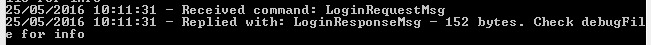
\includegraphics[width=1.0\linewidth]{figs/implementering/webtest}
	\caption{Web login forsøg}
	\label{fig:weblogintry}
\end{figure}

Testen bekræfter, at den generelle arkitektur for systemet virker sammen med ASP.NET MVC arkitekturen. 
\section{View}
\subsection{Windows GUI}
Til Windows er der udviklet et view-lag med WPF og C\#. Det findes under namespace "Smartpool.Application.Win."

\subsubsection{Design}
I Windows applikationen designes view-klasser, der implementerer view-interfacet defineret i præsentationslaget.
Designet af Windows GUI er lavet således, at codebehind filerne implementerer hver sit view-interfacet fra præsentationslaget. Codebehind agerer dermed som en bro, i mellem Smartpools præsentationslag, og WPF view-lag.

I klasse diagrammet nedenfor, ses Windows designet, af WinCreateUserView der implementerer ISignUpView fra applikationslaget og har en SignUpViewController.
\begin{figure}
	\centering
	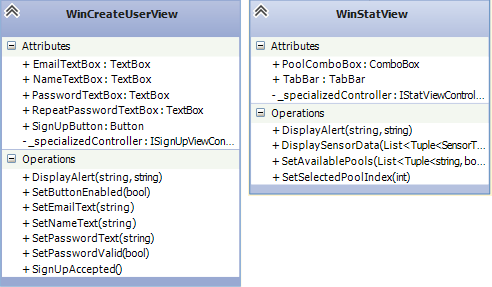
\includegraphics[width=0.7\linewidth]{figs/design/wincreateuserandwinstatviewview}
	\caption{WinCreateUserView og WinStatView}
	\label{fig:wincreateuserandwinstatviewview}
\end{figure}

Ligeledes er view klassen for WinStatView designet.
Klassen ses på figur~\ref{fig:wincreateuserandwinstatviewview}.

For yderligere forklaring se dokumentation afsnit Design under Windows.
\subsection{Windows GUI}
Til Windows er der udviklet et view-lag med WPF og C\#. Det findes under namespace "Smartpool.Application.Win."

\subsubsection{Design}
I Windows applikationen designes view-klasser, der implementerer view-interfacet defineret i præsentationslaget.
Designet af Windows GUI er lavet således, at codebehind filerne implementerer hver sit view-interfacet fra præsentationslaget. Codebehind agerer dermed som en bro, i mellem Smartpools præsentationslag, og WPF view-lag.

I klasse diagrammet nedenfor, ses Windows designet, af WinCreateUserView der implementerer ISignUpView fra applikationslaget og har en SignUpViewController.
\begin{figure}
	\centering
	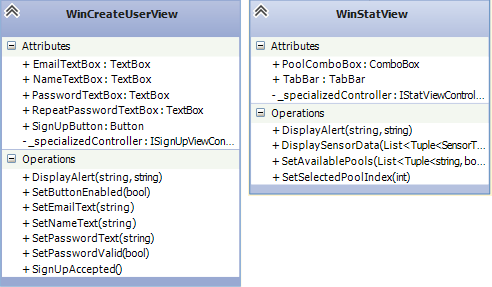
\includegraphics[width=0.7\linewidth]{figs/design/wincreateuserandwinstatviewview}
	\caption{WinCreateUserView og WinStatView}
	\label{fig:wincreateuserandwinstatviewview}
\end{figure}

Ligeledes er view klassen for WinStatView designet.
Klassen ses på figur~\ref{fig:wincreateuserandwinstatviewview}.

For yderligere forklaring se dokumentation afsnit Design under Windows.
\subsection{iOS}
I iOS applikationen designes view-klasser, der implementerer view-interfacet defineret i præsentationslaget. Det dominante user interface framework på iOS kaldes UIKit, og det er bygget op omkring en model-view-controller arkitektur. I UIKit har hvert view en tilhørende controller-klasse. I iOS designet tages der højde for dette, ved at bruge controller-klassen som en bro, i mellem Smartpools præsentationslag, og UIKits view-lag. Designet er derfor lavet således, at controller-klasserne på iOS implementerer view-interfacet fra præsentationslaget.

\subsubsection{SignUpViewBridge}
SignUpViewBridge-klassen implementerer ISignUpView interfacet. Klassen indeholder en række UIKit user interface elementer, som passer sammen med interfacet. Da dette view omhandler brugeroprettelse, er klassen designet til at indeholde en række tekstfelter, og en knap til at fuldende brugeroprettelsen. Denne klasse er designet til at nedarve fra UIKit klassen UIViewController, da de user interface elementer der indgår i designet, forventes at være statiske.

\begin{figure}
	\centering
	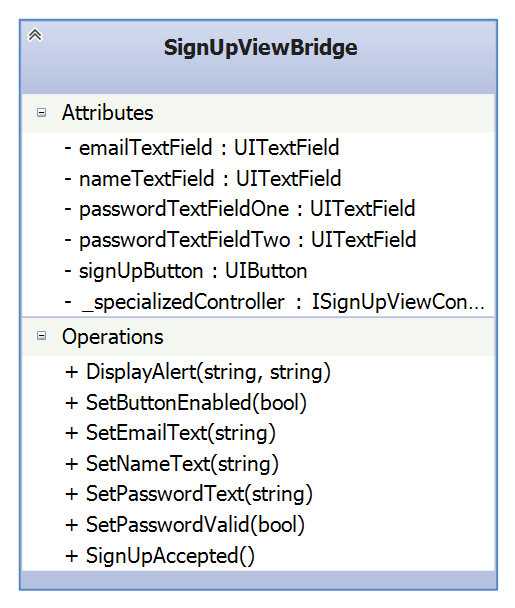
\includegraphics[width=0.3\linewidth]{figs/design/ios_signupviewbridge}
	\caption{SignUpViewBridge}
	\label{fig:ios_signupviewbridge}
\end{figure}

\subsubsection{StatViewBridge}
StatViewBridge-klassen implementerer IStatView interfacet. Dette view bør kunne håndtere dynamisk indlæsning og visning af måledata i følge de user stories, der er tilknyttet interfacet. Af denne grund nedarver StatViewBridge fra UITableViewController, der kan opsættes til at præsentere en dynamisk liste. StatViewBridge indeholder en UIBarButtonItem, der kan bruges til at skifte imellem pools i systemet.

\begin{figure}
	\centering
	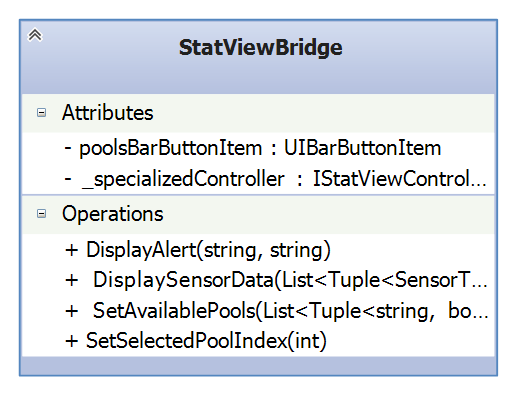
\includegraphics[width=0.3\linewidth]{figs/design/ios_statviewbridge}
	\caption{StatViewBridge}
	\label{fig:ios_statviewbridge}
\end{figure}
For yderligere forklaring se dokumentation afsnit Applikationslaget under Design.
\subsection{iOS}
I iOS applikationen designes view-klasser, der implementerer view-interfacet defineret i præsentationslaget. Det dominante user interface framework på iOS kaldes UIKit, og det er bygget op omkring en model-view-controller arkitektur. I UIKit har hvert view en tilhørende controller-klasse. I iOS designet tages der højde for dette, ved at bruge controller-klassen som en bro, i mellem Smartpools præsentationslag, og UIKits view-lag. Designet er derfor lavet således, at controller-klasserne på iOS implementerer view-interfacet fra præsentationslaget.

\subsubsection{SignUpViewBridge}
SignUpViewBridge-klassen implementerer ISignUpView interfacet. Klassen indeholder en række UIKit user interface elementer, som passer sammen med interfacet. Da dette view omhandler brugeroprettelse, er klassen designet til at indeholde en række tekstfelter, og en knap til at fuldende brugeroprettelsen. Denne klasse er designet til at nedarve fra UIKit klassen UIViewController, da de user interface elementer der indgår i designet, forventes at være statiske.

\begin{figure}
	\centering
	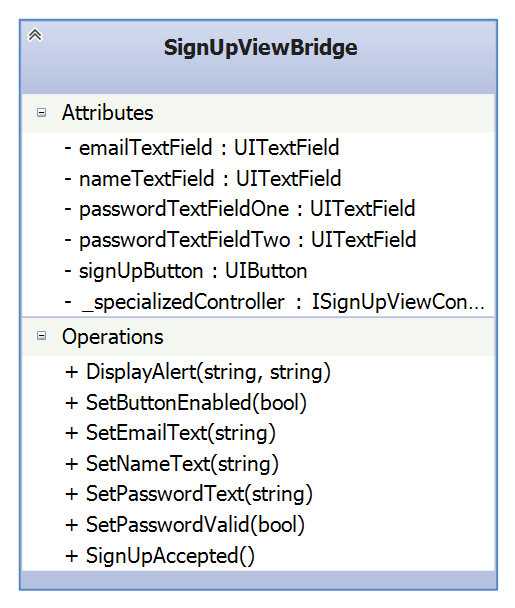
\includegraphics[width=0.3\linewidth]{figs/design/ios_signupviewbridge}
	\caption{SignUpViewBridge}
	\label{fig:ios_signupviewbridge}
\end{figure}

\subsubsection{StatViewBridge}
StatViewBridge-klassen implementerer IStatView interfacet. Dette view bør kunne håndtere dynamisk indlæsning og visning af måledata i følge de user stories, der er tilknyttet interfacet. Af denne grund nedarver StatViewBridge fra UITableViewController, der kan opsættes til at præsentere en dynamisk liste. StatViewBridge indeholder en UIBarButtonItem, der kan bruges til at skifte imellem pools i systemet.

\begin{figure}
	\centering
	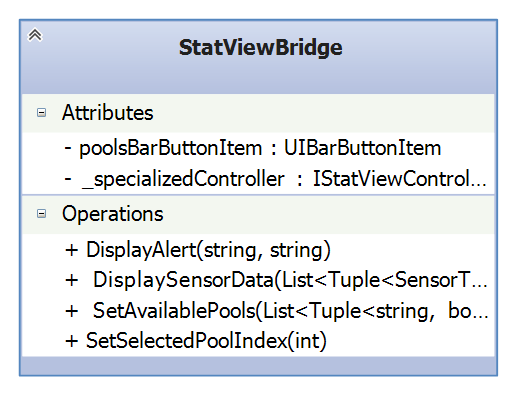
\includegraphics[width=0.3\linewidth]{figs/design/ios_statviewbridge}
	\caption{StatViewBridge}
	\label{fig:ios_statviewbridge}
\end{figure}
For yderligere forklaring se dokumentation afsnit Applikationslaget under Design.
% !TEX root = ../../I4PRJ, Grp3 - Rapport.tex
\subsubsection{Implementering}
Lorem ipsum
% !TEX root = ../../I4PRJ, Grp3 - Rapport.tex
\subsubsection{Implementering}
Lorem ipsum

% !TEX root = ../../../I4PRJ, Grp3 - Rapport.tex
\chapter{Grafisk Design}
I dette afsnit beskrives det grafiske design af brugergrænsefladen. Det grafiske design skal afspejle de respektive views funktionalitet. Først udarbejdes et konceptuelt design. GUI views designes ved at analyserer og diskuterer user stories for systemet. Resultatet af analysen er et håndtegnet design med tilhørende noter fra diskussionerne. Analyseresultatet dannede grundstenene for GUI folkenes arbejde. Designet blev dermed ensartet for de forskellige platforme. Det fælles udarbejdede design har mindsket en muligt senere kommende bureaukratisk proces, da alle udviklere ved at målet er nået, når GUI svarer til design. 

\section{Konceptuel Design}
Først udarbejdes et konceptuelt design. Det konceptuelle design udarbejdes ved analyse og diskussion af user stories, som eksempel er user story omhandlende login behandlet og kan ses på figuren nedenfor:

\begin{figure}
	\centering
	\includegraphics[width=\linewidth]{figs/design/konceptuel_design_loginview}
	\caption{Domænemodel for systemet}
	\label{fig:domainmodel}
\end{figure}

De forskellige platformes GUI minder i så høj grad om hinanden, at hvert view og hvilke user stories de implementerer kun vil blive beskrevet for en platform. 
\subsection{Farvepalet}
For at opfylde kvalitetskravet, at applikationer skal være visuelt ensartede, er der under det visuelle design lavet en Smartpool farvepalet.
\begin{table}[]
\centering
\begin{tabular}{ll}
SpBlack          & \cellcolor[HTML]{0A0A0A}{\color[HTML]{FFFFFF} \#FF0A0A0A} \\
SpDarkGrey       & \cellcolor[HTML]{1F1F1F}{\color[HTML]{FFFFFF} \#FF1F1F1F} \\
SpGrey           & \cellcolor[HTML]{575757}{\color[HTML]{FFFFFF} \#FF575757} \\
SpLightGrey      & \cellcolor[HTML]{ABABAC}\#FFABABAC                        \\
SpOrange         & \cellcolor[HTML]{FDA029}\#FFFDA029                        \\
SpRed            & \cellcolor[HTML]{FF584D}\#FFFF584D                        \\
SpLightBlue      & \cellcolor[HTML]{49BAE1}\#FF49BAE1                        \\
SpBlue           & \cellcolor[HTML]{0354A5}\#FF0354A5                        \\
SpWhite          & \cellcolor[HTML]{FFFFFF}\#FFFFFFFF                        \\
SpBackgroundGray & \cellcolor[HTML]{2E2E2E}{\color[HTML]{FFFFFF} \#FF2e2e2e} \\
SpAccentGray     & \cellcolor[HTML]{3E3E3E}{\color[HTML]{FFFFFF} \#FF3e3e3e}
\end{tabular}
\caption{Farvepalet}
\label{table:farvepalet}
\end{table}

\section{Forbindelse}
\chapter{Fremtidigt arbejde}

\section{Connection}

\subsection{Overordnet connection struktur}
\textbf{Klient} delen består af et model projekt som er generelt for alle platforme, samt et klient projekt som er specifikt for hver platform. Dette er gjort for at gøre så meget som muligt anvendeligt på alle platforme. I model projektet er desuden defineret en række besked objekter, som anvendes ved kommunikation mellem klient og server.
\textbf{Server} delen består af en række systemer som tilsammen udgør en samlet server udviklet til at køre på en windows pc. Al kommunikation til databasen foregår fra server delen.

\subsection{Klient}
Klienten modtager besked objekter fra applikations laget, og omdanner disse til en streng vha. Json serializering. Strengen bliver sendt til server delen gennem en socket klient der passer til den pågældende platform.
Klienten modtager derefter et svar fra serveren, i form af et serializeret besked objekt, som bliver deserializeret til basis besked klassen. Denne indeholder en besked type, og klienten kan derefter deserializere den modtagne streng til det korrekte besked objekt. Derefter bliver objektet sendt videre, tilbage til applikations laget. 

\subsection{Server}
Vedligeholder følgende funktioner i systemet
\begin{itemize}
	\item Modtage, behandle og svare på requests fra klient delen
	\item Varetage user sessions
	\item Kommunikere med databasen via metoder i database delen
	\item Simulere pool data
\end{itemize}

\subsubsection{Modtage, behandle og svare på requests fra klient delen}
Serveren modtager via en Asyncronous Socket Client (ASC) en streng fra klient delen. Denne bliver, som i klienten, lavet til et basis besked objekt. Denne bliver derefter behandlet vha. en switchcase, hvor der reageres på hvilken message type der er blevet sendt. Dette foregår i en ResponseManager klasse, og denne vil, i nogle situationer, være i stand til selv at udføre den kaldte request. Det gør den ved f.eks. at lave et kald til databasen og returnere svaret derfra. 
I andre situationer, bliver kaldet sendt videre til en sub handler, som f.eks. TokenMsgResponse, der tager sig af alle requests, som kræver at brugeren er logget ind. Dette er lavet således at ResponseManager checker, via databasen, om brugeren er logget ind, og hvis dette er tilfældet, bliver beskeden sendt videre til TokenMsgResponse. TokenMsgResponse behøver dermed ikke selv at kontrollere om brugeren er logget ind.
Hvis beskedtypen ikke genkendes, sendes svar tilbage til klienten om dette.

\subsubsection{User sessions}
For at holde styr på hvilke brugere som er logget ind, er der udviklet et Token system. Dette system giver en øget sikkerhed, ved at brugeren kun sender password en enkelt gang, og det behøver derfor heller ikke at blive gemt i klienten. Desuden bliver der færre kald til databasen, da efterfølgende requests ikke behøver at kontrollere brugerens password via databasen.
Token systemet virker ved at en bruger, ved login, får tilknyttet en streng af tilfældige karakterer. Brugernavnet bliver, sammen med strengen af karakterer og et timestamp, gemt i en klasse der hedder Token. Alle disse tokens bliver så vedligeholdt i en TokenKeeper. Når en bruger efterfølgende laver en request til serveren, sender klienten både username og token strengen med i sin request. Serveren kontrollerer derefter om dette stemmer overens med de data som ligger i TokenKeeperen, samt om det gemte timestamp er ældre end systemets valgte sessions tid.
En bruger kan godt være logget ind på flere enheder på samme tid. I det tilfælde vil hver enhed få tildelt en token streng, og dermed har de ikke indflydelse på hinandens session.

\subsubsection{Kommunikere med databasen via metoder i database delen}
Serveren kommunikerer via tilgængelige metoder i systemet dataaccess layer ??

\subsubsection{Simulerering af pool data}
Da Smartpool systemet ikke anvender reele data, er der udviklet en FakePool klasse til at simulere dette. Denne opretter en af hver type sensor. Hver sensor bliver initieret med en værdi, der ligger indenfor et realistisk område, for den pågældende sensor type. 
Denne værdi opdateres med et angivet internal, hvorefter værdierne gemmes i databasen. Værdi opdateringen foregår med små tilfældigt genererede ændringer. Disse er yderligere begrænset af en minimum og maximum grænse, specificeret i en SensorValueAuthenticator klasse.  


\section{Data}
\todo{Skriv indledning til Data}
\chapter{Fremtidigt arbejde}

\section{Database og Data Access Layer}

Der er med udgangspunkt i designovervejelserne i afsnit~\ref{sec:designdatabase} implementeret et fungerende data-access layer med tilhørende database.

\subsection{Implementering af database}

Databasen er implementeret med en Model First tilgang \cite{microsoftdatadevelopercenter2016}. Det vil sige at der opsættes en model (ER diagram) for databasen i Visual Studio, hvorefter der genereres et SQL script der kan køres mod den specifikke database. Scriptet køres mod en tom database, hvor de opstillede entities genereres som tabeller.

Data entiteten som ses på figur~\ref{fig:datasetentity} da bruges som en klasse, se klassedigram på figur~\ref{fig:efGeneratedData}. De forskellige datatyper, pH, chlorine, temperature og humidity figurerer som lister (ICollections) i Data klassen. Disse lister er i koden angivet som virtual. Dette er for at gøre lazy loading muligt, hvilket betyder at de først bliver loadet fra databasen når de tilgås gennem deres navigation property \cite{microsoftdevelopernetwork2016} (linje 7 i listing~\ref{code:chlorinecode}).

Som det kan ses på figur~\ref{fig:datasetentity}, har diverse datatyper (Chlorine, Ph...) en \textit{DataId} property. Denne bruger til at identificere hvilket \textit{DataSet} den enkelte måling høre til. På denne måde behøver de enkelte datatyper ikke selv at have et \textit{Timestamp} medlem. 

\begin{figure}[h]
	\centering
	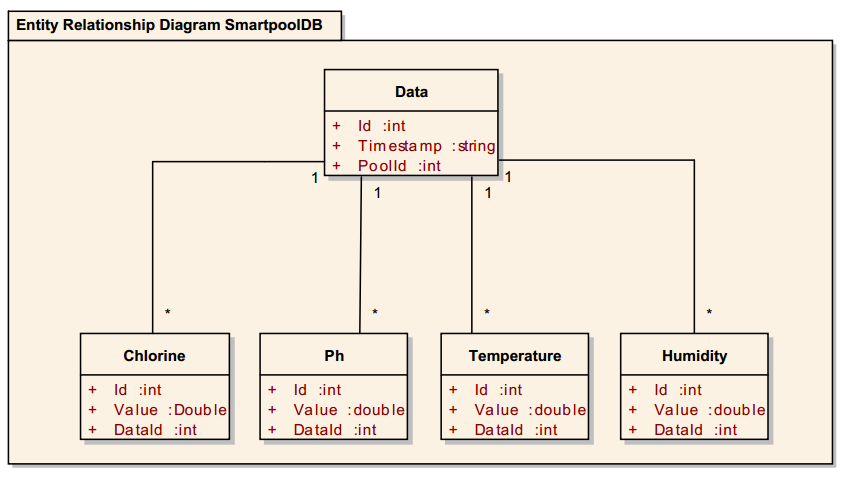
\includegraphics[width=0.8\linewidth]{figs/implementering/datasetentity.png}
	\caption{Data Entity fra ER diagrammet i Visual Studio}
	\label{fig:datasetentity}
\end{figure}

Når \gls{ef} oversætter ER diagrammet til C\# kode og laver scriptet, bliver eksempelvis Chlorine Entity'en til C\# koden vist i listing~\ref{code:chlorinecode}. I dette kodesnit kan man se hvordan \gls{ef} har givet \textit{Chlorine} klassen en \textit{virtual Data}, som et eksempel på lazy loading anvendt.

\begin{minipage}[h]{\linewidth}
\begin{lstlisting}[caption=C\# kode repræsentationen af Chlorine entity.,label=code:chlorinecode]
public partial class Chlorine
{
	public int Id { get; set; }
	public double Value { get; set; }
	public int DataId { get; set; }
	
	public virtual Data Data { get; set; }
}
\end{lstlisting}
\end{minipage}

\begin{figure}
	\centering
	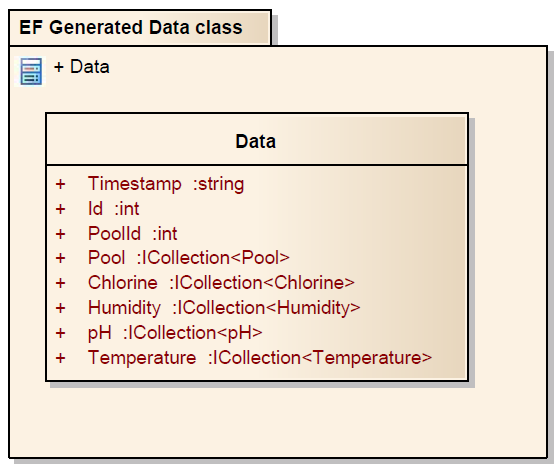
\includegraphics[width=0.5\linewidth]{figs/implementering/efGeneratedData.PNG}
	\caption{Data klassen - Genereret fra Entity Model}
	\label{fig:efGeneratedData}
\end{figure}

\subsection{Implementering af data-access layer}

Entity Frameworket er et \textit{object-relational mapping} framework. Det giver mulighed for at oprette et database-kontekst objekt. Ændringer/indsætning af data sker gennem dette objekt. Når der ønskes en query på databasen gøres det i projektet ved hjælp af en LINQ\footnote{Language Integrated Query} query på en af kontektsobjektets properties. Disse properties er af typen \textit{DbSet<T>} som er en samling af alle entiterne, T i konteksten. Resultatet en af query kan da behandles i en foreach løkke.

For at give et indblik i implementeringen, kan der nedenfor ses kodeudsnit, som tager udgangspunkt i to af projektets user stories, herunder tilføjelse af bruger samt at visning af pooldata.

\subsubsection{Træk pooldata ud}

\textit{"Som bruger vil jeg kunne se de seneste sensor værdier for at kunne få et overblik over poolens tilstand"}\

I de følgende kodeudsnit vises der med tilhørende forklaring hvordan data kan udtages fra databasen. I dette eksempel bruges metoden \textit{GetChlorineData()}, en dybdegående forklaring af alle \textit{Get..Data} metoder kan findes i dokumentationen \todo{reference til dokumentation}.

<<<<<<< HEAD

=======
>>>>>>> ead435153a2f8ba0e8b66926208049c0ba0f7dfb
\begin{lstlisting}[caption=GetChlorineData method - konvertering af DateTime objekter, label=code:getChlorineData]
public List<Tuple<SensorTypes, double>> GetChlorineValues(string poolOwnerEmail, string poolName, int daysToGoBack)
{
	double days = System.Convert.ToDouble(daysToGoBack);
	string now = DateTime.UtcNow.ToString("G");
	string start = DateTime.Parse(now).AddDays(-days).ToString("G");
	...
\end{lstlisting}

På kodeudsnit \ref{code:getChlorineData} vises måden hvorpå et UTC timestamp oprettes. Der benyttes UTC tid da al data gemmes på én server. Det er derfor ligegyldigt hvor i verden en måling bliver foretaget, da dens timestamp vil følge UTC. Det nuværende tidspunkt skal bruges da meningen med funktionen er at returnere alt klor-data der er målt i tidsperioden angivet som \textit{daysToGoBack} parameteren. DateTime \cite{dotnetdatetime} klassen er en del af .NET og indeholder informationer om klokkeslet og dato. Antallet af dage der skal samles informationer om fratrækkes den nuværende DateTime. Derved fås startdatoen til data queryen. Strengen G der medgives som parameter til \textit{ToString}, bevirker at formateringen af tid og dato bliver \textit{dd/MM/yyyy HH:mm:ss}

\begin{lstlisting}[caption=Konvertering tilbage til DateTime objekter,label=code:convertToDateTime]
using (var db = new DatabaseContext())
		{   
			DateTime startTime = DateTime.ParseExact(start, "dd/MM/yyyy HH:mm:ss", System.Globalization.CultureInfo.InvariantCulture);
			DateTime endTime = DateTime.ParseExact(now, "dd/MM/yyyy HH:mm:ss", System.Globalization.CultureInfo.InvariantCulture);

			var chlorineDataQuery = from chlorine in db.ChlorineSet
					where chlorine.Data.Pool.Name == poolName && chlorine.Data.Pool.User.Email == poolOwnerEmail
					select chlorine;

\end{lstlisting}

Som det kan ses på kodeudsnit \ref{code:convertToDateTime} konverteres timestamp strengene til DateTime objekter, hvorefter der bruges LINQ til at lave en forespørgsel på klor-data. Bemærk at der kun hentes klor-data for én specifik bruger og en enkelt af brugerens pools.

\begin{lstlisting}[caption=Iteration over indhentet pool data,label=code:dataIteration]
List<Tuple<SensorTypes, double>> chlorineTuples = new List<Tuple<SensorTypes, double>>();

foreach (var chlorine in chlorineDataQuery)
{
	if(DateTime.Parse(chlorine.Data.Timestamp).CompareTo(endTime) < 0 ||
	DateTime.Parse(chlorine.Data.Timestamp).CompareTo(startTime) > 0)
	{
		chlorineTuples.Add(new Tuple<SensorTypes, double>(SensorTypes.Chlorine, chlorine.Value));
	}
}

return chlorineTuples;
\end{lstlisting}

Returtypen på metoden er en liste af tupler, hvor hver tuple repræsenterer en måling. Som det kan ses på kodeudsnit \ref{code:dataIteration} sammenlignes den data som blev hentet i kodeudsnit \ref{code:convertToDateTime} med de to DateTime objekter, \textit{endTime} og \textit{startTime}. På denne måde gemmes de relevante klor data som tupler i listen.

\subsubsection{Tilføj user}

\textit{"Som bruger vil jeg kunne oprette mig i systemet for at få adgang til systemet"}

I de følgende kodeudsnit vises der med tilhørende forklaringer hvordan en bruger bliver oprettet og gemt i databasen. Der tages udgangspunkt i metoden \textit{AddUser}, som er en del af UserAccess\footnote{Se dokumentationen XXXX} klassen. AddUser metoden kaldes af ConnectionServer klassen \todo{indsæt kodeudsnit af kald her!} som set på figur XXXX.
 
\begin{lstlisting}[caption=User laves lokalt hvorefter User's navne properties sættes, label=code:adduser1]
public bool AddUser(string fullname, string email, string password)
{
	...
	//Checks for existing user and valid name
	...
	
	User user;

	string[] names = fullname.Split(' ');

	if (names.Length <= 2)
	{
		user = new User() { Firstname = names[0], Lastname = names[1], Email = email, Password = password };
	}
	else
	{
		user = new User() { Firstname = names[0], Middelname = names[1], Lastname = names[2], Email = email, Password = password };
	}
\end{lstlisting}

Som det kan ses på kodeudsnit \ref{code:adduser1} Oprettes en user først lokalt, hvorefter user objektets navne, password og email properties sættes. En User's navn opdeles i Firstname, Middlename og Lastname strings. 

\begin{lstlisting}[caption=User objektet tilføjes i database konteksten hvorefter der gemmes på selve databasen,label=code:adduser2]
	using (var db = new DatabaseContext())
	{
		db.UserSet.Add(user);
		db.SaveChanges();
	}

	return true;
}
\end{lstlisting}

Når der skal foretages ændringer på databasen, oprettes et database kontekst objekt hvor ændringerne gemmes på. Derefter kaldes \textit{db.SaveChanges()} metoden, som gemmer ændringerne på selve databasen. Se kodeudsnit \ref{code:adduser2} for eksempel på brugen af database konteksten med \textit{using} direktivet.


	\clearpage %% Design
	
	\chapter{Fremtidigt arbejde}
			\clearpage %% Resultater
	\chapter{Fremtidigt arbejde}
	\clearpage %% udviklingsværktøjer
	\chapter{Fremtidigt arbejde}
		\clearpage %% Fremtidigt arbejde
	\chapter{Fremtidigt arbejde}
			\clearpage %% Konklusion
	\chapter{Fremtidigt arbejde}
				\clearpage %% Appendix
	
	\backmatter
	\setglossarystyle{list}
	\printnoidxglossary[title=Ordliste]		%% Glossary
	
	\clearpage
	\printbibliography[title={Litteratur}] 	%% Bibliography
\end{document}